\subsection{Example - Simple}
The following is a very basic grammar definition for gt. When completed the 
grammar will allow for one to many ID's where each is separated by a PLUS (eg. x + x). 
This example can be found in \textit{gt/tests/bnf/simple.gra}. 

First, a name for your grammar will need to be defined. A grammar name is the first declaration in a gt
definition. It starts with a lowercase letter that is followed
by zero or many upper- or lowercase letters, underscores and/or numbers (['a'-'z' 'A'-'Z']
['0'-'9' '\_' 'a'-'z' 'A'-'Z' ]*). We will name this grammar \textit{simple}.

The next part of the grammar file that can be defined is the line\_comment delimiter.
This definition is optional. If the there is not a line\_comment definition the default
definition will be used -- \textit{\#}.\\
\begin{gt}
simple

line_comment = "%".
\end{gt} 

The next step in creating a grammar definition is to define the productions. A production consists of a
constructor name, type name and elements. The production name is a unique identifier and should
start with an uppercase letter. These are used by gt to define the corresponding OCaml constructors for
the syntax trees parsed. A production also has a type name which should start with a lowercase letter. The 
type names do not have to be unique and are used by gt to name the corresponding OCaml types. Lastly, 
the elements of a production are a sequence of lexical, type names or nothing. These productions are used
to declare OCaml types that will then be used to parse to syntax trees. \\
\begin{gt}
Expr : expr -> ID PLUS expr.
Id : expr -> ID.
\end{gt} 

The last step in creating a grammar is to define the lexical classes. The above example used ID and PLUS as
some of the elements in the productions. To define the lexical classes the user must first decide what they want 
ID and PLUS to represent. To make it simple this example defined ID to be an \textit{x} and PLUS to be a \textit{+}.
Putting all of this together we get the following grammar definition.\\
\begin{gt}
simple

line_comment = "%".

Expr : expr -> ID PLUS expr.
Id : expr -> ID.

PLUS = "+".
ID = "x".
\end{gt} 

% Generated Functions
\subsubsection{Generated Functions}
The files that are generated by gt for this grammar start with \textit{simple}. For example, the equality function
is called \textit{simple\_eq.ml} which is shown below. The equality function takes in a 
pair and returns true if the two elements in the pair are equal otherwise it returns false. The type for the equality 
function is $ ('a * 'a) \rightarrow bool $. \\
\lstinputlisting[language=ML]{./examples/bnf/simple/simple_eq.ml}\ \\
%
%
\noindent Another file that is outputted by gt is the file containing the pretty printer function.
As the name implies, pretty printer helps print the parsed program in a readable format. Instead of
printing out the text that the generated parser has after creating the syntax trees, this function 
preserves the newlines of the original file. However, the pretty printer does not preserve 
comments, tabs or spaces. Below is the pretty printer definition for this example, \textit{simple\_pp.ml}.\\
%
%
\lstinputlisting[language=ML]{./examples/bnf/simple/simple_pp.ml}\ \\
\noindent The following is the output for the function that creates a Graph-Viz file. This function
will create a visual representation of a syntax tree for a program that is parseable by the generated 
parser. \\
\lstinputlisting[language=ML]{./examples/bnf/simple/simple_gviz.ml}

% Syntax Trees
\subsubsection{Syntax Trees}


Now that the parser for the given file has been generated by gt it is ready to be used. 
Figure 2.3 shows the syntax tree that is generated by the above grammar.
%
%
%
\begin{figure}[h!]
  \centering
  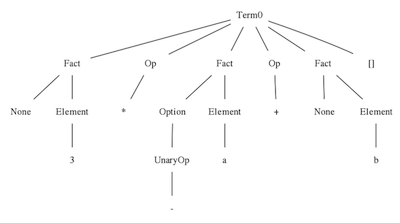
\includegraphics[width=4in]{./examples/ebnf/arith/ebnf-arith.png}
  \caption{Syntax Tree for\\ \textit{3 * -a + b}}
\end{figure}

